\documentclass[tikz,border=10pt]{standalone}
\usepackage{amsmath}
\usepackage{amssymb}
\usepackage{tikz}
\usetikzlibrary{arrows.meta,calc}

\definecolor{figazul}{RGB}{2,132,199}
\definecolor{figrojo}{RGB}{220,38,38}
\definecolor{figverde}{RGB}{22,163,74}

\begin{document}
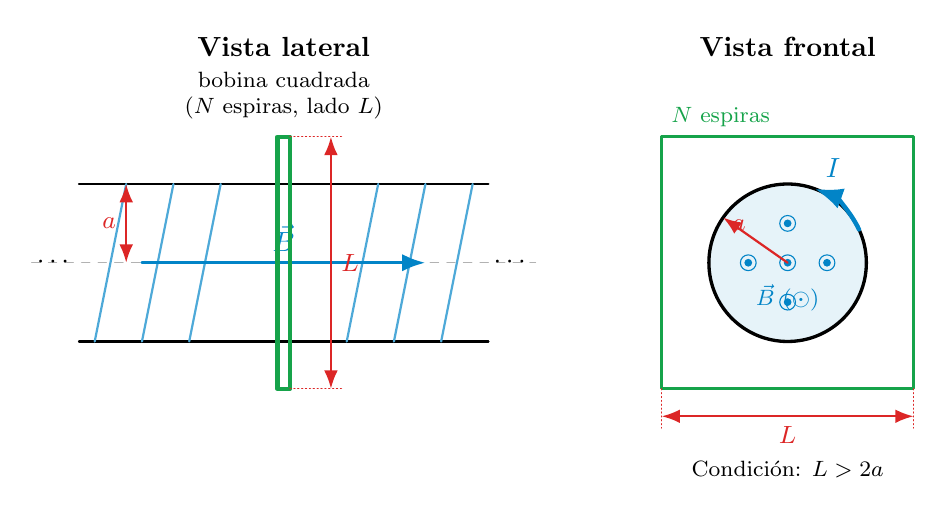
\begin{tikzpicture}[>=Latex, line cap=round, line join=round]
  % -------------------------------------------------------------
  % Panel Izquierdo: Vista lateral
  % -------------------------------------------------------------
  \begin{scope}[xshift=0cm]
    \node[above, font=\bfseries] at (0, 2.5) {Vista lateral};

    % Eje horizontal longitudinal del solenoide
    \draw[dashed, color=gray!60] (-3.2, 0) -- (3.2, 0);

    % Contorno del solenoide de radio a = 1.0
    \draw[thick] (-2.6, 1.0) -- (2.6, 1.0);
    \draw[thick] (-2.6, -1.0) -- (2.6, -1.0);
    \node at (-2.9, 0) {$\cdots$};
    \node at (2.9, 0) {$\cdots$};

    % Espiras del solenoide (trazos inclinados regulares)
    \foreach \x in {-2.2, -1.6, -1.0, 1.0, 1.6, 2.2} {
      \draw[thick, color=figazul!70] (\x-0.2, -1.0) -- (\x+0.2, 1.0);
    }

    % Línea de campo B en el interior
    \draw[->, very thick, color=figazul] (-1.8, 0) -- (1.8, 0) node[above, midway, color=figazul] {$\vec{B}$};

    % Bobina cuadrada central de lado L = 3.2 (perfil: de y = -1.6 a y = 1.6 en x = 0)
    \draw[ultra thick, color=figverde] (-0.08, -1.6) rectangle (0.08, 1.6);
    \node[above, font=\footnotesize, align=center] at (0, 1.7) {bobina cuadrada\\($N$ espiras, lado $L$)};

    % Cota del radio a del solenoide (en rojo)
    \draw[<->, thick, color=figrojo] (-2.0, 0) -- (-2.0, 1.0) node[midway, left, color=figrojo, font=\small] {$a$};

    % Cota del lado L de la bobina cuadrada (en rojo)
    \draw[<->, thick, color=figrojo] (0.6, -1.6) -- (0.6, 1.6) node[midway, right, color=figrojo, font=\small] {$L$};
    \draw[densely dotted, thin, color=figrojo] (0.08, 1.6) -- (0.75, 1.6);
    \draw[densely dotted, thin, color=figrojo] (0.08, -1.6) -- (0.75, -1.6);
  \end{scope}

  % -------------------------------------------------------------
  % Panel Derecho: Vista frontal
  % -------------------------------------------------------------
  \begin{scope}[xshift=6.4cm]
    \node[above, font=\bfseries] at (0, 2.5) {Vista frontal};

    % Bobina cuadrada exterior de lado L = 3.2
    \draw[very thick, color=figverde] (-1.6, -1.6) rectangle (1.6, 1.6);
    \node[above right, font=\footnotesize, color=figverde] at (-1.6, 1.6) {$N$ espiras};

    % Sección circular del solenoide de radio a = 1.0
    \draw[very thick, fill=figazul!10] (0, 0) circle (1.0);

    % Flecha de corriente I en sentido antihorario
    \draw[->, ultra thick, color=figazul] (25:1.0) arc (25:70:1.0) node[above right, color=figazul] {$I$};

    % Campo B saliente (\odot) dentro del solenoide
    \foreach \ang in {0, 90, 180, 270} {
      \draw[thin, color=figazul] (\ang:0.5) circle (0.10);
      \fill[color=figazul] (\ang:0.5) circle (1.4pt);
    }
    \draw[thin, color=figazul] (0, 0) circle (0.10);
    \fill[color=figazul] (0, 0) circle (1.4pt);
    \node[below, font=\footnotesize, color=figazul] at (0, -0.15) {$\vec{B}$ ($\odot$)};

    % Cota del radio a (en rojo)
    \draw[->, thick, color=figrojo] (0, 0) -- (145:1.0);
    \node[above left, color=figrojo, font=\small] at (145:0.5) {$a$};

    % Cota del lado L (en rojo)
    \draw[<->, thick, color=figrojo] (-1.6, -1.95) -- (1.6, -1.95) node[midway, below, color=figrojo, font=\small] {$L$};
    \draw[densely dotted, thin, color=figrojo] (-1.6, -1.6) -- (-1.6, -2.1);
    \draw[densely dotted, thin, color=figrojo] (1.6, -1.6) -- (1.6, -2.1);

    % Nota L > 2a
    \node[below, font=\footnotesize] at (0, -2.4) {Condici\'on: $L > 2a$};
  \end{scope}
\end{tikzpicture}
\end{document}
